\chapter{Implementation}\label{chap:Implementation}

In this section, we will discuss the implementation of each of the components of libbind. The workflow/usage is covered separately in Chapter~\ref{chap:Workflow}. Any major deviations from what has been covered in Design and Architecture will be highlighted.

\section{Binary Abstraction Layer}

\begin{figure}[H]
 \centering
 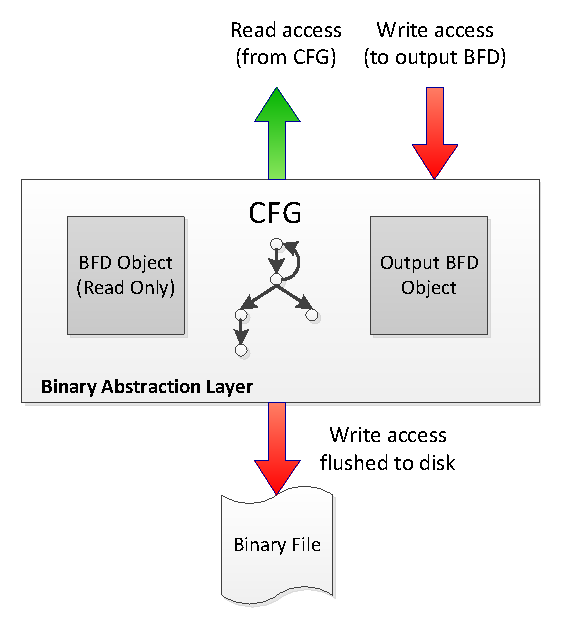
\includegraphics{Binary_Abstraction_Layer_Attempt1.pdf}
 \caption{The original approach for the binary abstraction layer. The read only BFD object is the abstraction of the original binary file. The CFG is generated from this BFD. Any changes need to be outputted to the output BFD independently.}
\label{fig:BAL_Attempt1}
\end{figure}

The binary abstraction layer was originally designed to act as a bridge between the components and the target file. Essentially, libbind encapsulates a binary file in an internal structure called a \emph{bin\_file}. A \emph{bin\_file} contains two important elements: the BFD abstraction of a binary and its corresponding CFG (which is generated by the static analysis engine). In general, when a component needs to read information about the binary, it will read from the generated CFG. As we have seen, writing to the binary is equivalent to modifying the CFG. After a change to the CFG occurs, this change is flushed to the underlying binary through the BFD object. This was the original concept but it had to be modified to work in practice. Figure~\ref{fig:BAL_Attempt1} illustrates the original approach to creating the binary abstraction layer.

\subsection{Original Approach}

The problem with the original design was that it only encapsulated a single BFD object. With libbfd, it is possible to open a file in two ways:

\begin{enumerate}
\item An existing file can be opened with read-only access.
\item A \emph{new and empty} file can be opened with write access.
\end{enumerate}

This restriction of libbfd is by design, but does not make it ideal for patching. Tools such as \emph{ld} and \emph{objcopy} work well above libbfd because the files they output are written in a single pass. Although BFD is unsuitable for our usage, it is possible (albeit very awkward) to patch a binary file. Figure~\ref{fig:BAL_Approach1} illustrates the steps required to patch a file through libbfd:

\begin{figure}[H]
 \centering
 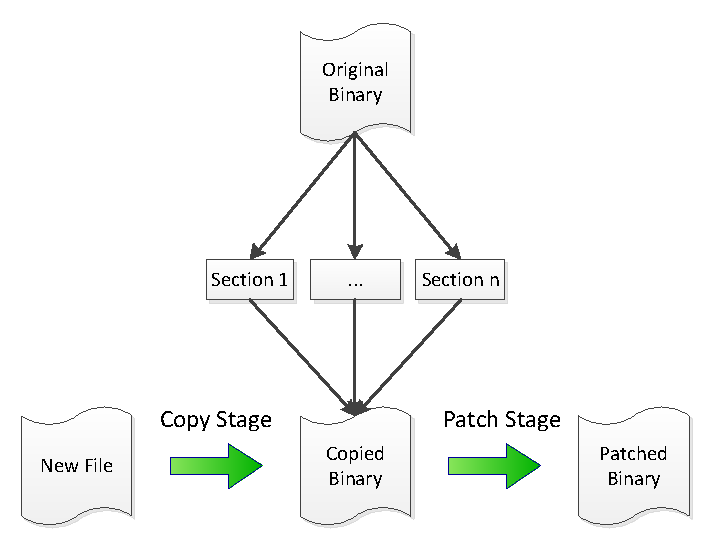
\includegraphics{Binary_Abstraction_Layer_Approach1.pdf}
 \caption{The process required to patch a file using libbfd.}
\label{fig:BAL_Approach1}
\end{figure}

The abstraction used within BFD is that an object file has:

\begin{itemize}
\item A header
\item A number of sections containing raw data (this data could represent code)
\item A set of relocations
\item Symbol information
\end{itemize}

As illustrated, patching a binary file with libbfd works through a series of steps:

\begin{enumerate}
\item The original binary must first be opened with read access.
\item A new BFD (which starts off empty) is created. The original binary is then reconstructed in this BFD by extracting the four different types of content (as defined above) and copying them. This reconstruction all happens in memory.
\item Before the new BFD object is flushed to disk, the user is able to perform patches by editing the contents of sections.
\item After all patches are performed, the BFD object is flushed to disk. If more modifications are needed after this, the entire process has to be restarted.
\end{enumerate}

In terms of the implementation of this algorithm, the first two stages are essentially what objcopy does. Our implementation of static patching re-uses the objcopy code for the decomposition and reconstruction stage. The rest of the algorithm is trivial to implement. However, there are two drawbacks with this method:

\begin{enumerate}
\item The part of the code re-used from objcopy is large, approximately 1.5 KLOC.
\item BFD is merely an abstraction over many file formats. This means that it represents a more generalised abstract format. Unfortunately, it does not encapsulate all the information required for the full reconstruction of a binary. In order to obtain this information, the code relies on a dependency with the file format and ends up calling functions in libelf.
\end{enumerate}

\subsection{Final Approach}

\begin{figure}[H]
 \centering
 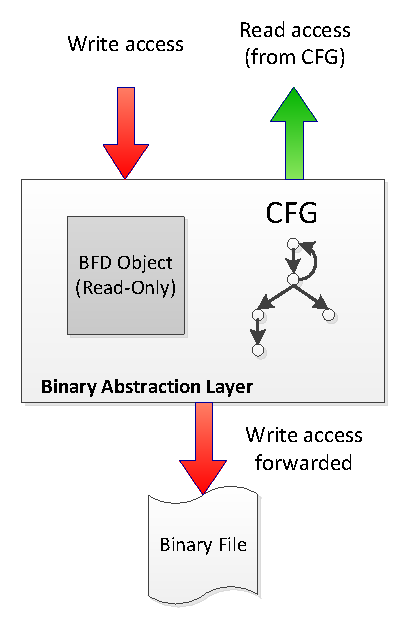
\includegraphics{Binary_Abstraction_Layer_Final.pdf}
 \caption{The final design for the binary abstraction layer. Read accesses are handled in the same way but in this design, we have removed the output BFD. Write accesses alter the target binary file directly.}
\label{fig:BAL_Final}
\end{figure}

Given the disadvantages of using the method from the original approach, there is no reason to use BFD to perform the patching. The method is overly complicated and more error-prone simply because of the amount of code that has to be written to perform a patch. Since a dependency on libelf is unavoidable, we can re-implement the solution by using libelf directly and save the hassle of forcing libbfd to do something it was not designed for. In terms of the binary abstraction layer, this means that we modify write accesses to directly modify the disk version instead of through the BFD object as seen in Figure~\ref{fig:BAL_Final}.
 
In the final implementation of the binary abstraction layer where libelf is used, the same result as with the original approach can be achieved in under 100 LOC. The method is fairly intuitive and the concept is visualised in Figure~\ref{fig:Loading_Binary}:
 
\begin{figure}[H]
 \centering
 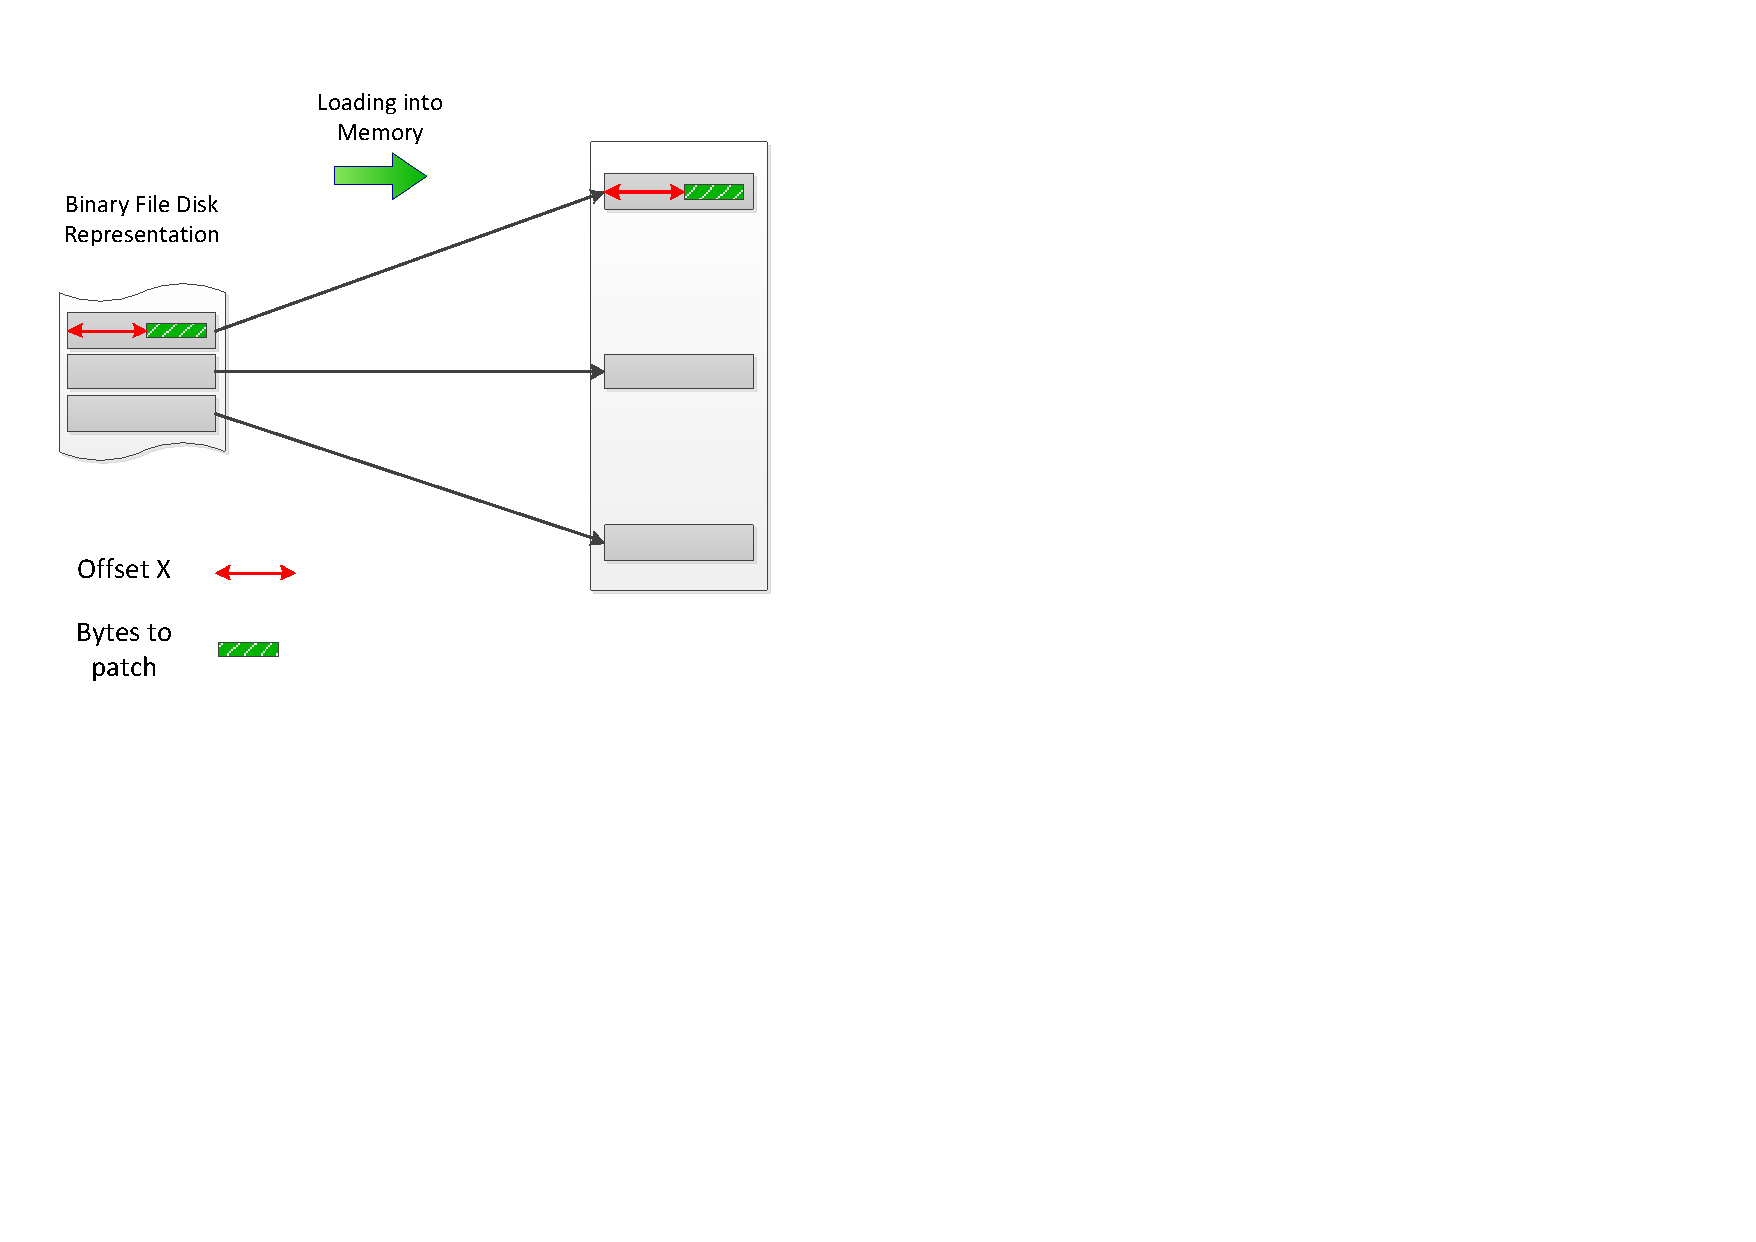
\includegraphics{Loading_Binary.pdf}
 \caption{The concept of how patching works in the final implementation. The most important idea here is that a section in the disk representation is preserved (not split) when it is mapped into memory. This means data that is at a certain offset into the section in the disk representation will be offset by the same amount after loaded into memory.}
\label{fig:Loading_Binary}
\end{figure}
 
In libelf, similarly to libbfd, an executable contains a set of sections in which both code and data can reside. When the operating system loads the executable into memory, each section is based at some base address. We can reverse this to map a virtual memory address to a physical file offset. If a physical file offset can be found, the bytes can be patched as a regular file.

\begin{enumerate}
\item First, the section header of the executable is parsed with libelf. This allows us to obtain a set of sections and most importantly, for each section libelf can tell us three things:
  \begin{description}
  \item [Section size] The size of the section.
  \item [Section base address] The address that the section will be based at when the executable on disk is loaded into memory.
  \item [Section disk offset] The disk offset of the section.
  \end{description}
\item By iterating through the section information extracted in the previous step, it is possible to find out what section an arbitrary virtual memory address is contained in. During patching, the memory address we are interested in is the address of the code at which a detour is to be written. The offset of the virtual memory address into the section can be calculated by:

\textbf{(virtual\_memory\_address - section\_base\_address)}.
\item Therefore, the disk offset of the virtual memory address can be calculated by:

\textbf{(section\_disk\_offset + (virtual\_memory\_address - section\_base\_address))}.
\end{enumerate}

This process allows an arbitrary virtual memory address to be mapped to its corresponding disk file offset. This offset can then be patched with regular C file IO functions such as \emph{fopen}/\emph{fseek}/\emph{fwrite}/\emph{fclose}.

Fortunately the architecture of libbind was designed such that a change in the implementation of one component (even if that is the binary abstraction layer) would not impact the other components. The downside is that a lot of time was lost writing the BFD patch code, only to have it thrown out in favour of another method. However, this was unavoidable as the documentation did not make it clear how difficult the implementation of patching would be. The lack of clear documentation is a widely recognised drawback to libbfd and the required steps were only discovered by reading through the objcopy source.

\section{Static Analysis Engine}

As discussed in earlier sections, the static analysis engine allows libbind to discover the code of a binary. It is implemented in several layers and matches the design described in Design (Chapter~\ref{chap:Design}). Figure~\ref{fig:SAE_Detail} shows the internal implementation of the static analysis engine in more detail:

\begin{figure}[H]
 \centering
 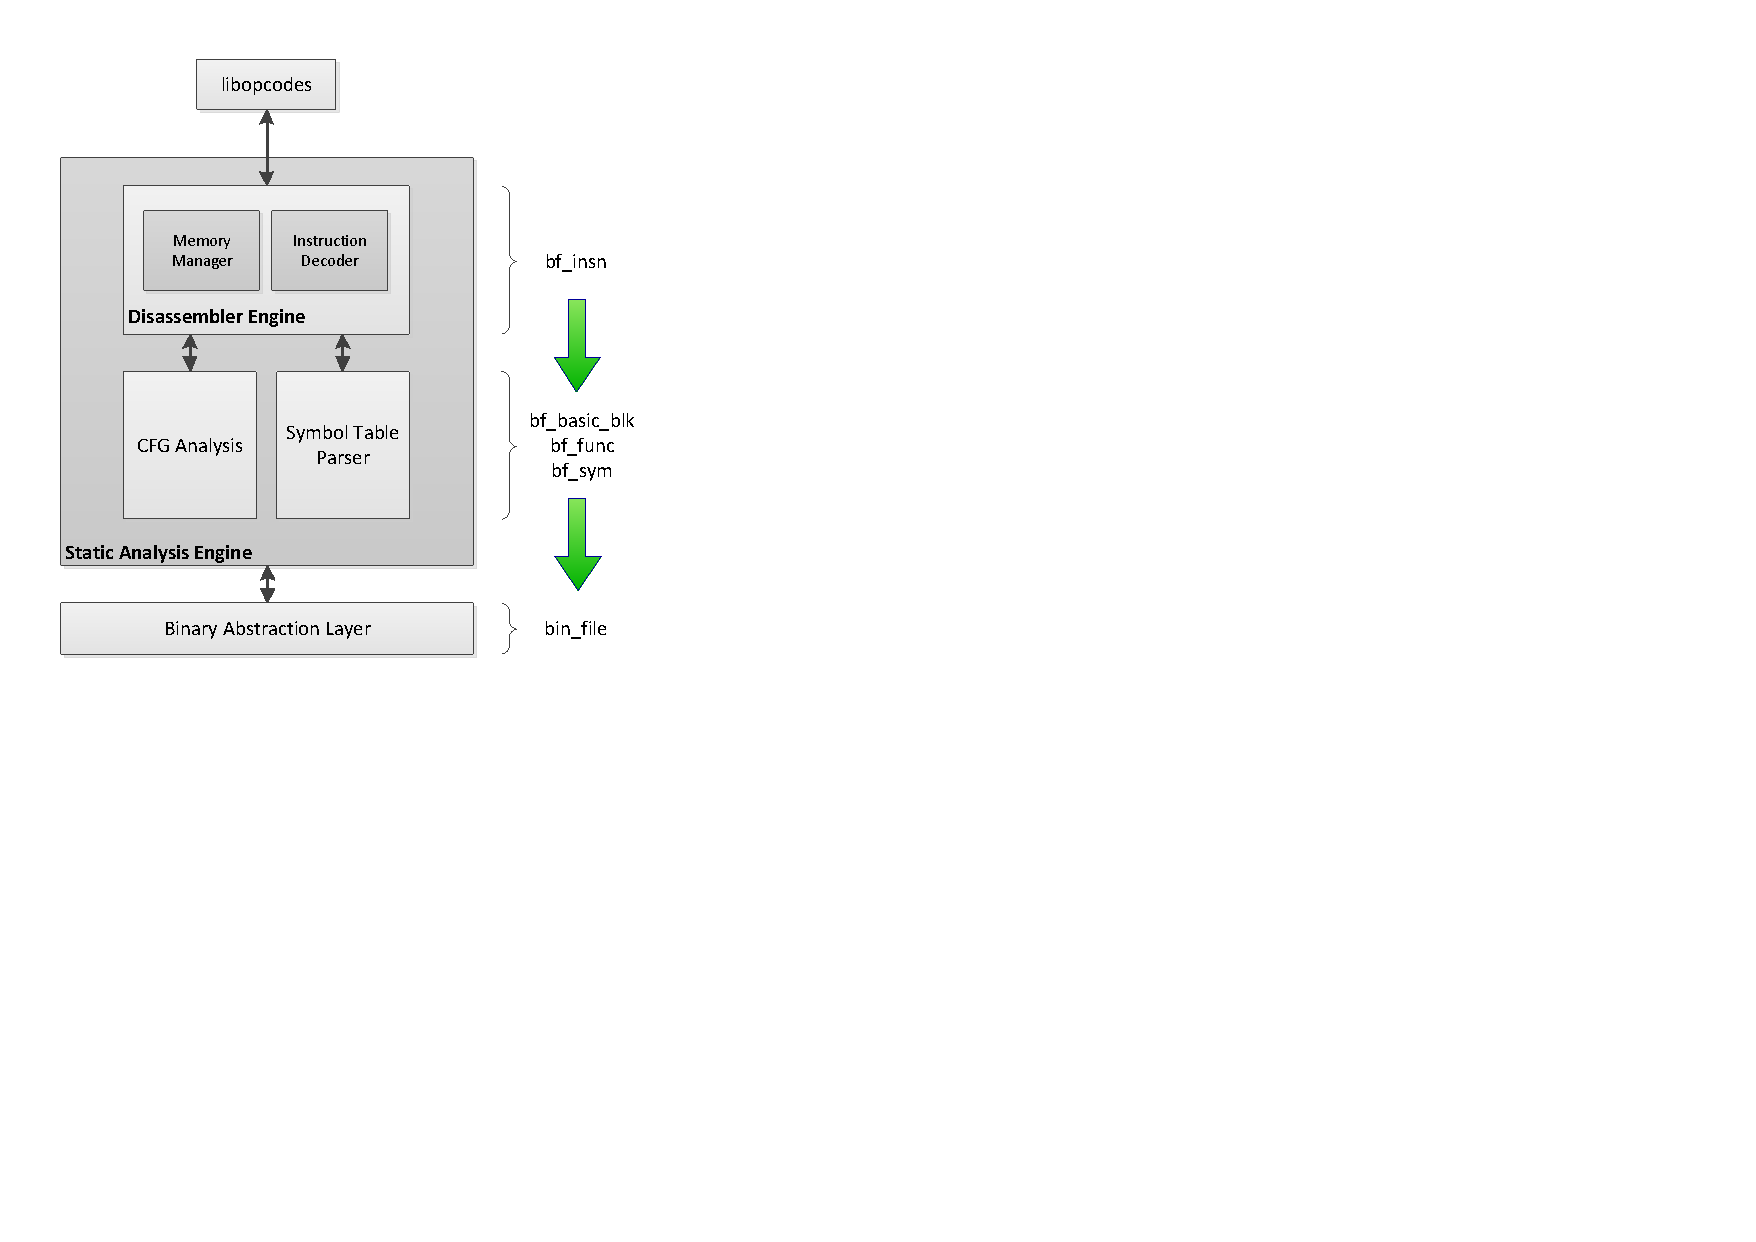
\includegraphics{Static_Analysis_Engine_Detail.pdf}
 \caption[Hierarchy]{The internal implementation of the static analysis engine.}
\label{fig:SAE_Detail}
\end{figure}

From a high level, the disassembler engine builds bf\_insn objects to represent each disassembled instruction. The CFG analysis drives the disassembler engine to identify basic block boundaries and to generate the CFG. A CFG is simply a graph of bf\_basic\_blk objects. Certain bf\_basic\_blk objects correspond to the start of a function and can be additionally labelled as bf\_func objects. The symbol table parser attaches symbol information to the generated CFG by associating bf\_sym objects with the relevant bf\_basic\_blk objects.

In order to understand how the static analysis engine works as a whole, we will explain each component in further detail.

\subsection{Disassembler Engine}

In practice, the disassembler engine is responsible for parsing and translating the strings received from libopcodes and storing the information in its internal semantic representation. At the most basic level, a \emph{bf\_insn} corresponds to an assembly instruction. In order to use libopcodes, we first needed to solve the two problems outlined in Design:

\begin{description}
\item [Limited disassembly scope] libopcodes can only disassemble a single address at a time which means the same applies for the disassembler engine. In order to make the disassembler engine useful, CFG analysis needs to be performed when an instruction is disassembled. The results of this analysis will then be used to drive the disassembler engine. For example, if the CFG analysis comes across a conditional branch instruction, it will need to instruct the disassembler engine to disassemble both the branch target and the next instruction. This analysis will be covered in detail later since it is not part of the disassembler engine.
\item [Output redirection] The default behaviour of libopcodes is to print to a stream using \emph{fprintf}. It is possible to override this behaviour by instructing libopcodes to invoke a custom function with the same prototype as fprintf.
\end{description}

One quirk of libopcodes is that it invokes the fprintf function (or overridden substitute) for each of the following `types': mnemonic, operand, separator and comment. As a concrete example, consider the following instruction:

\noindent\begin{minipage}{\textwidth}
\begin{lstlisting}[language={[x86masm]Assembler},caption={Example instruction disassembled by libopcodes.}]
ucomiss 0x9124(%rip), %xmm0 # 414d58
\end{lstlisting}
\end{minipage}

The custom fprintf function is invoked 6 times with the following:

\noindent\begin{minipage}{\textwidth}
\begin{lstlisting}[language={[x86masm]Assembler},caption={Strings received by custom fprintf. Type information is included for the benefit of the reader but is not given by libopcodes.}]
ucomiss (Mnemonic)
0x9124(%rip) (Operand)
, (Separator)
%xmm0 (Operand)
# (Separator)
414d58 (Comment)
\end{lstlisting}
\end{minipage}

The main goal of the disassembler engine is to take these inputs and produce something useful which can be used for CFG analysis. One option is to concatenate all these instruction parts to obtain a full instruction but we already decided in Design that we would not store instructions in string from. The main problem with storing strings is that semantic information needs to be extracted as part of the CFG analysis anyway. Furthermore, users of the library would need to reproduce the exact same extraction code. One advantage of storing strings is that it is convenient for printing instructions. This means an instruction decoder must be able to:

\begin{description}
\item [Map instruction parts to semantic information] For example, instead of the string \enquote{\$0x3ef}, its parsed value (0x3ef) should be stored.
\item [Map the stored semantic information back to its string equivalent] For example, it should be possible for a mnemonic such as \enquote{mov} to be stored semantically (perhaps as an enum) as part of the first requirement. Mapping back to its string equivalent means mapping the enum value back to a string.
\end{description}

The implementation stores semantic information about each instruction by decoding each part as it is received from libopcodes. The decoded information is stored in a bf\_insn object corresponding to the current address being disassembled. An issue with this approach is that libbind needs to know how to decode every type of string it receives. For example, an arbitrary string that is received might be a mnemonic, operand, separator or comment which all need to be decoded in different ways. It would be very inefficient to attempt to decode each string to determine what type it should be. libbind solves this issue by implementing a finite state machine (Figure~\ref{fig:Instruction_State_Machine}) which allows it to know what type it is expecting to receive next.

Each time a new instruction is disassembled, a new bf\_insn object is constructed and the current state is restarted to the initial state of the instruction finite state machine. When fprintf is called, the received string is decoded based on its expected type, the semantic information updated for the bf\_insn and the current state of the state machine advanced. $S_1$ is a special case because two types can be received at this point: an operand or a mnemonic. In this case, we can only decode as one type and if that fails decode as the other type. Since an operand is more common, the disassembler engine attempts to decode as that first. The implementation of the instruction decoder is covered later.

\begin{figure}[H]
 \centering
 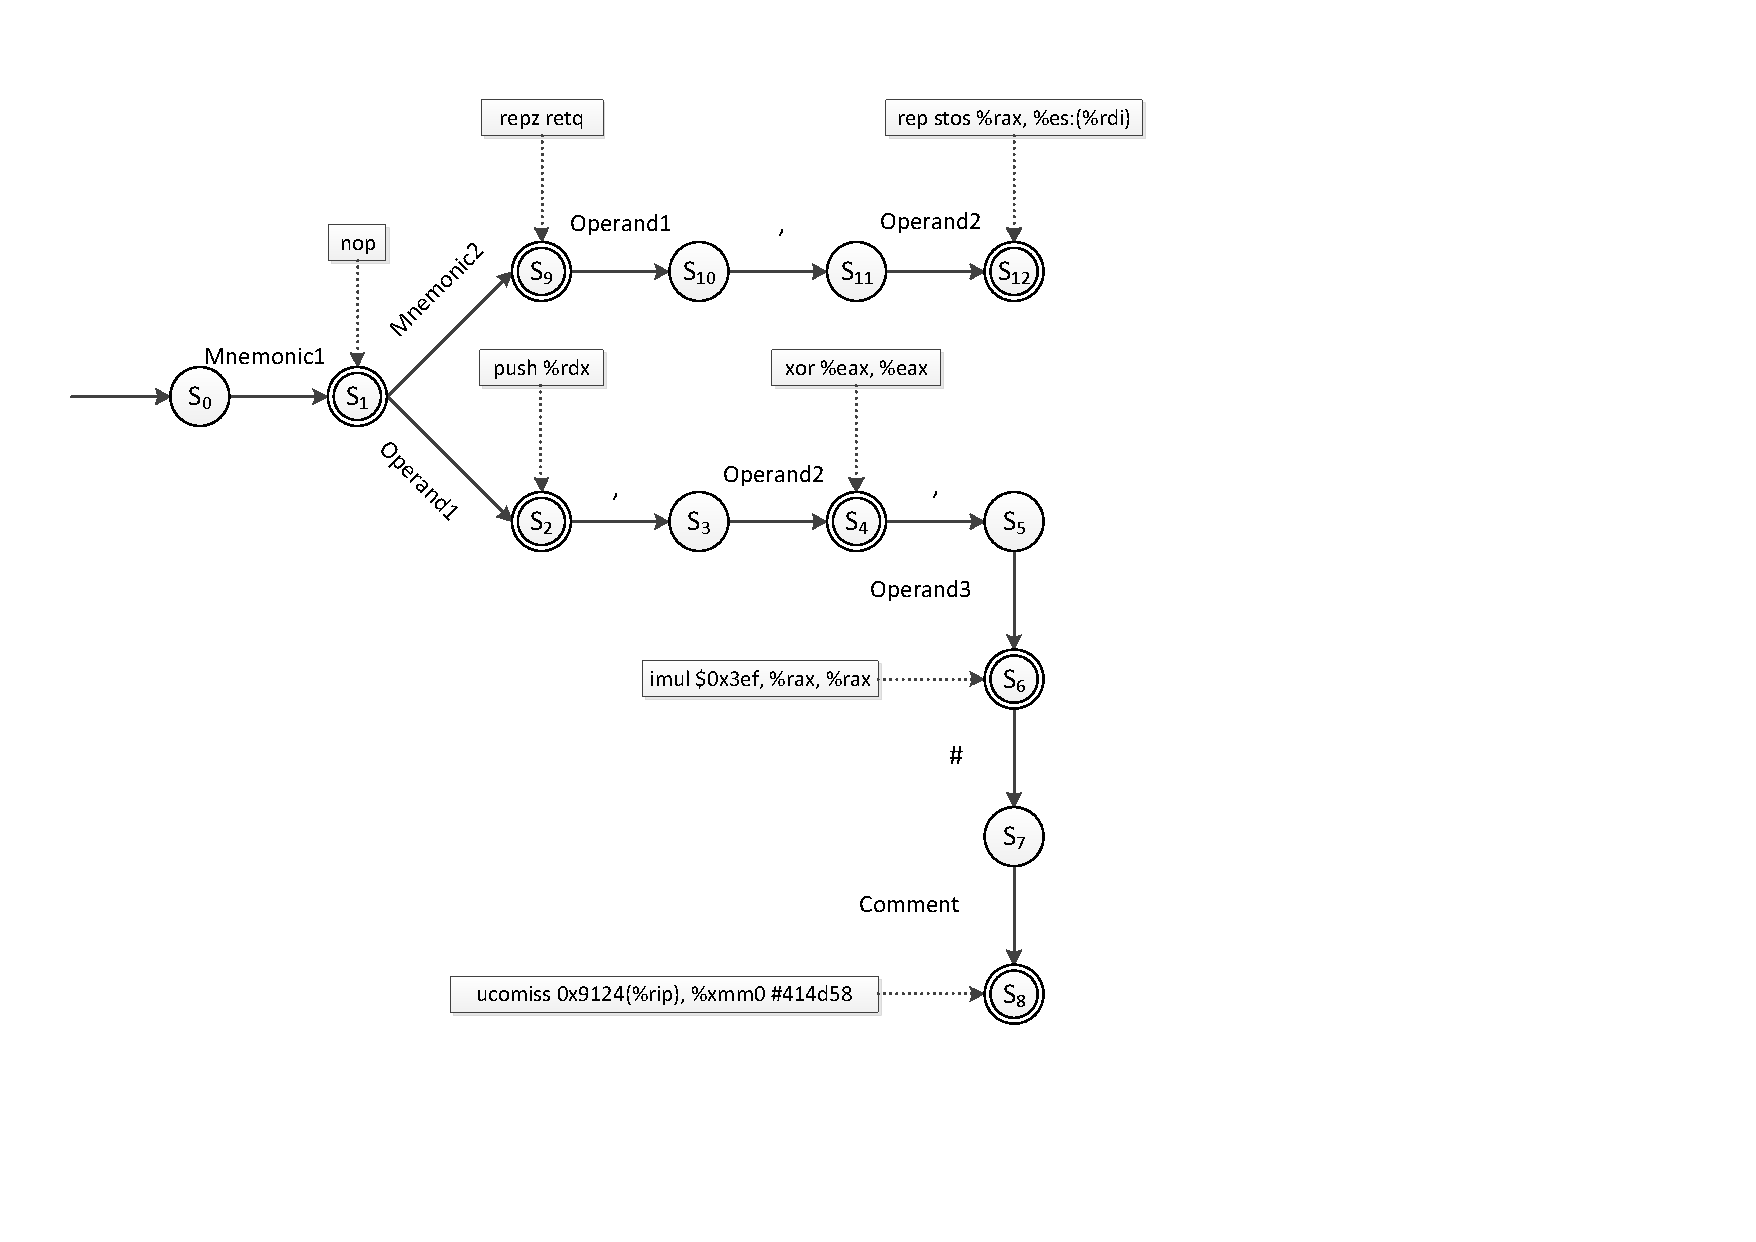
\includegraphics[scale=0.9]{Instruction_State_Machine.pdf}
 \caption[Hierarchy]{The instruction finite state machine used by the disassembler engine to determine how the received string should be decoded. A double circle denotes a possible terminal state. For each terminal state, an example instruction which would cause termination at that state is shown.}
\label{fig:Instruction_State_Machine}
\end{figure}

\subsubsection{Memory Manager}

From an architectural point of view, the memory manager does not play an important role. It is discussed here briefly for completeness. Under the BFD abstraction, all data (including code) resides in a section. The vast majority of interactions involving data, including disassembling with libopcodes, requires the section containing the data to be loaded. The libopcodes/libbfd interface then requires a pointer to the section object. In order to make the API of libbind as lightweight as possible, it was decided that the concept of a section should be abstracted because it should not be necessary for a user to know about them. This means the disassembler engine is invoked without section information. The memory manager intercepts all requests sent to the disassembler and examines the target address being disassembled. It then loads the appropriate section, adds this information and then forwards the request to libopcodes. For efficiency, the memory manager only unloads sections during the final cleanup when a bin\_file is closed which means no section is ever loaded more than once.

\subsubsection{Instruction Decoder}

The two key aims of the instruction decoder have been discussed already, but to briefly recap, the instruction decoder is responsible for:

\begin{itemize}
\item Mapping strings representing instruction parts to a semantic representation.
\item Mapping this semantic representation back to string form for printing.
\end{itemize}

We maintain that a semantic representation is a more natural way of working with assembly instructions as opposed to string comparisons. However, it is also understandable that people would want to use strings either out of preference and habit or in order to print onto the screen. This is why we require the mapping to go both ways. A further requirement is that any solution for the instruction decoder needs to be highly efficient and have minimal overhead, particularly to go from string to semantic representation since this is part of the disassembling process as seen above.

Every string received from libopcodes needs to be decoded which means there are four cases to handle:

\begin{description}
\item [Mnemonics] \enquote{mov}, \enquote{xor}, \enquote{repz}, \ldots
\item [Operands] \enquote{\%rax}, \enquote{\%es:(\%rdi)}, \enquote{0x9124(\%rip)}, \ldots
\item [Separators] \enquote{,} and \enquote{\#}
\item [Comments] \enquote{414d58}, \enquote{602030}, \ldots
\end{description}

We will enumerate how each case is handled starting from the most basic case.

\paragraph{Separators}

A separator is defined either as \enquote{,} or \enquote{\#}. This is the most simple case to handle. When the instruction decoder encounters a separator, it simply does nothing since this information does not need to be stored semantically. The disassembler will automatically advance the instruction finite state machine and the next part of the instruction will be decoded.

\paragraph{Comments}

Comments are extra information added by libopcodes that suggest the value of an operand. They always appear in the form of a hexadecimal value without the 0x prefix. These can be decoded without effort with \emph{sscanf} with the \emph{\%lx} format specifier.

\noindent\begin{minipage}{\textwidth}
\paragraph{Operands}

Instruction operands are represented in bf\_insn objects by a struct containing a union (Listing~\ref{lst:insn_operand}).

\noindent\begin{minipage}{\textwidth}
\begin{lstlisting}[language=C,caption={The insn\_operand struct which holds the semantic representation of operands within instructions.},label=lst:insn_operand]
struct insn_operand {
	enum operand_type tag;
	union {
		bfd_vma		    val;
		uint64_t	    imm;
		bfd_vma		    addr_ptr;    
		enum insn_reg	    reg;
		enum insn_reg	    reg_ptr;
		struct array_index  arr_index;
		struct array_index  arr_index_ptr;
		uint64_t	    index_into_fs;
		struct cs_index	    index_into_cs;
		enum insn_reg	    index_into_es;
		enum insn_reg	    index_into_ds;
		bfd_vma		    index_into_gs;
	} operand_info;
};
\end{lstlisting}
\end{minipage}

All the different cases need to be enumerated when performing the decoding:

\begin{quote}
\begin{description}
\item [Values] 0x9124, 0x2348098, \ldots
\item [Immediates] \$0x8f0a, \$0x3ef, \ldots
\item [Address Pointers] *0x8f0a, *0x3ef, \ldots
\item [Array Indexes] 0x200c2a(\%rip), -0x28(\%rsp), 0x0(\%rax,\%rax,1), \ldots
\item [Array Index Pointers] *0x200c2c(\%rip), *0x600e28(,\%rax,8), *(\%r12,\%rbx,8), \ldots
\item [Index into CS/ES/DS/GS] \%cs:0x0(\%rax,\%rax,1), \%es:(\%edi), \%ds:(\%rsi), \ldots

These operands can be decoded trivially by pattern matching with \emph{sscanf}. When an operand consists of the conjunction of several types, the decoding is performed recursively. For example, decoding $0x0(\%rax,\%rax,1)$ requires $0x0$, $\%rax$, $\%rax$ and $1$ to be decoded.

\item [Registers] \%rax, (\%bl), (\%r14b), \ldots
\item [Register Pointers] *\%rax, *\%rbx, *\%rcx, \ldots

Registers and register pointers are decoded in the same way as mnemonics. The reasoning behind this will become clear in the explanation of mnemonic decoding.
\end{description}
\end{quote}
\end{minipage}

\paragraph{Mnemonics}

The decoding of mnemonics is the most tricky case. The most appropriate/intuitive C data type to be used for the representation of mnemonics is the enumerated type. Classically, a string can be mapped to an enumerated type and vice versa as shown by Listing~\ref{lst:classical_enum}. The forward case (string to enum) uses string comparisons and has a running time complexity of \emph{O(n)}\footnote{We ignore the complexity of the strcmp operation by assuming each strcmp takes the same amount of time. We are interested only in complexity with respect to the number of separate cases in the \emph{switch..case} statement.}. The backward case (enum to string) uses \emph{switch..case} and has a running time complexity of \emph{O(1)} in the best case\footnote{Switch/case is usually optimised to O(1), but this is not defined by the C standard. In practice, GCC generally makes the O(1) optimisation based on a threshold of three or more case parts (excluding the default).} 

It is worth noting that efficiency for the forward case is more important than for the backward case. That is, users generally care more about the speed of disassembly than the time taken to print or dump instructions. While the classical implementation is trivial to implement, it should be possible to improve on the forward case complexity of \emph{O(n)}.

\noindent\begin{minipage}{\textwidth}
\begin{lstlisting}[language=C,caption={Classical implementation for mapping strings to enumerated type and vice versa.},label=lst:classical_enum]
/*
 * Running time complexity of O(n).
 */
enum insn_mnemonic str_to_mnemonic(char * str)
{
	enum insn_mnemonic = 0;
	
	if(strcmp(str, "aaa") == 0) {
		insn_mnemonic = aaa_insn;
	} else if(...) {
		insn_mnemonic = ...
	} else if(strcmp(str, "xorps") == 0) {
		insn_mnemonic = xorps_insn;
	}

	return insn_mnemonic;
}

/*
 * Running time complexity of O(1).
 */
char * mnemonic_to_str(enum insn_mnemonic mnemonic)
{
	char * str = NULL;
	
	switch(mnemonic) {
	case aaa_insn:
		str = "aaa";
		break;
	
	case ...		
	
	case xorps_insn:
		str = "xorps";
		break;

	default:
	}
	
	return str;
}
\end{lstlisting}
\end{minipage}

One way to reduce the forward case complexity is to create a perfect hash function, which maps all possible mnemonic strings to \emph{unique} enum values. There exist tools such as GNU gperf for generating perfect hash functions but this approach is brittle and rigid to change. The x86 instruction set has been extended many times throughout its history with many of these additions occuring with the release of a specific processor. Updating libbind under such scenarios would require regeneration of the perfect hash function.

libbind extends the concept of using a perfect hash function by using an approach which aims to be more amenable to change and minimise the cost of the hash overhead. The decoding of mnemonics is done by generating an enumerated type where the values of members correspond to the integer representation of the mnemonic string representation as shown in Listing~\ref{lst:mnemonic_str_int}.

\noindent\begin{minipage}{\textwidth}
\begin{lstlisting}[language=C,caption={Example mnemonic string and integer representations.},label=lst:mnemonic_str_int]
enum insn_mnemonic {
	mov_insn = (uint64_t)`m' | (uint64_t)`o' << 8 | (uint64_t)`v' << 16,
	ret_insn = (uint64_t)`r' | (uint64_t)`e' << 8 | (uint64_t)`t' << 16,
	sysenter_insn = (uint64_t)`s' | (uint64_t)`y' << 8 | (uint64_t)`s' << 16 |
		(uint64_t)`e' << 24 | (uint64_t)`n' << 32 | (uint64_t)`t' << 40 |
		(uint64_t)`e' << 48 | (uint64_t)`r' << 56
};
\end{lstlisting}
\end{minipage}

The bit-shifting is abstracted through a macro which allows the same enumeration to be defined as follows:

\noindent\begin{minipage}{\textwidth}
\begin{lstlisting}[language=C,caption={Macro abstraction.}]
enum insn_mnemonic {
	mov_insn = INSN_TO_ENUM('m','o','v'),
	ret_insn = INSN_TO_ENUM('r','e','t'),
	sysenter_insn = INSN_TO_ENUM('s','y','s','e','n','t','e','r')
};
\end{lstlisting}
\end{minipage}

In libbind, the insn\_mnemonic enumeration is actually generated by passing a list of mnemonics to a Java program which acts as a pre-preprocessor to generate the C enumeration. However, it is clear that adding a new instruction in this implementation is trivial. This approach allows the forward stage to be defined as so:

\noindent\begin{minipage}{\textwidth}
\begin{lstlisting}[language=C,caption={Forward stage.}]
enum insn_mnemonic mnemonic = 0;
strncpy((char *)&mnemonic, str, sizeof(uint64_t));
\end{lstlisting}
\end{minipage}

The backward stage is defined as so:

\noindent\begin{minipage}{\textwidth}
\begin{lstlisting}[language=C,caption={Backward stage (mnemonic is of type \emph{enum insn\_mnemonic}). The extra byte in the char array is used as padding for the null terminator.}]
char str[sizeof(uint64_t) + 1] = {0};
memcpy(str, &mnemonic, sizeof(uint64_t));
\end{lstlisting}
\end{minipage}

As a side-note, it may appear at a first glance that the backward stage can alternatively be defined equivalently as the following:

\noindent\begin{minipage}{\textwidth}
\begin{lstlisting}[language=C,caption={mnemonic is of type \emph{enum insn\_mnemonic}. The array str is casted to a pointer to a uint64\_t and assigned the value of mnemonic.}]
char str[sizeof(uint64_t) + 1] = {0};
*(uint64_t *)str = mnemonic;
\end{lstlisting}
\end{minipage}

However this code is not standards complaint because of the type-punning. Such an implementation is illegal and violates strict aliasing rules. It would result in undefined behaviour because a pointer is dereferenced that aliases another of an \emph{incompatible type}. The standards compliant way of performing the assignment is with memcpy. Empirically, GCC often compiles the two code snippets into identical assembly code by optimising the memcpy, but it is important that we do not rely on this behaviour since it is not defined by the standard.

The approach taken by libbind satisfies the following prerequisites:

\begin{description}
\item [Efficiency] Both the forward and backward mapping are \emph{O(1)}. On top of this, the implementation amounts to copying 8 bytes of memory with no extra calculations. It is unlikely any generated hash function would be able to beat this.
\item [Uniqueness] Every mnemonic in the x86 instruction set is uniquely identifiable from its first 8 characters. There are three exceptions where the mnemonic length is longer than 8 bytes (namely \emph{cvttsd2si}, \emph{cvttss2si} and \emph{cvtsi2sdq}). These special cases are handled by manually truncating the \emph{INSN\_TO\_ENUM} macro input.  \emph{cvttsd2si} and \emph{cvttss2si} can not simply be truncated because the first 8 characters are shared so they are arbitrarily assigned different values. These special cases are checked in both the forward and backward cases to ensure that correct observable behaviour is preserved.
\end{description}

As mentioned during discussion of the operand decoder, registers are decoded in the same way as mnemonics, but stored in a separate enumeration (\emph{enum insn\_reg}). In order to analyse instructions easier, libbind exposes functions to get more information about enumeration values. For example, functions to check if a mnemonic represents an instruction which will break flow (an unconditional branch), branch flow (a conditional branch or \emph{loop} mnemonic), call subroutines (\emph{call}/\emph{callq}) or end flow (\emph{ret}, \emph{sysret}, etc.).

The implementation of mnemonic decoding described above has portability implications which are discussed in Writing Standards Compliant Code (Section~\ref{sec:standards_compliance}). This discusses how the approach relies on implementation-defined behaviour of GCC (which affects the portability of libbind across different compilers).

\subsection{CFG Analysis}

A control flow graph represents a binary file using graph notation where nodes are basic blocks. There are many control flow analysis algorithms used to generate the CFG of a program. The vast majority of these build on top of the same basic algorithm to analyse the structure of a binary but differ in how hard they try to reach higher levels of coverage. In general, this corresponds to how much effort is put into performing analysis on indirect branching and indirect procedure invocation\cite{cfg}. Static analysis is not the main goal of this project so we did not aim to maximise coverage. Instead, we establish a basic awareness of the general techniques available and ensure the CFG analysis code we write is amenable to extensions (such as support for indirect branch analysis). To demonstrate this, we implement a proof of concept example of one case of indirect branching. This shows that extending the CFG analysis of libbind to be more powerful in the future is feasible.

The aim of the CFG analysis in libbind is to generate a basic CFG, ignoring indirect branching. The purpose of the generated CFG is to help users locate and identify source and destination basic blocks for detours and trampolines. Instead of building our own CFG analysis, we could have used existing libraries but in the general case, they build above their own disassembler engine. We wanted to be able to use our own disassembler engine to have tighter control over the interface and the library architecture without having to wrap an existing library. A further advantage of using our own disassembler engine is that we can control the implementation. We take advantage of this by using our own instruction decoder to completely eliminate the use of strings.

In our CFG analysis, we consider only direct branching and direct calls. What this means is that indirect calls due to function pointers or jump tables can not be resolved. For this reason, analysing programs with characteristics such as packing or polymorphism will not produce useful results. As part of its API, libbind gives the user the ability to dump part of or the whole of a CFG. We will use these dumps to demonstrate how the analysis works.

\subsubsection{CFG Generation Algorithm}

The CFG analysis is a recursive process for detecting basic blocks and is defined as so:

%\begin{enumerate}
%\item The disassembly is started from a root. This is typically the entry point.
%\item A new bf\_basic\_blk object is created and associated with the current address being disassembled. The CFG analysis then drives the disassembler engine in a linear fashion. This means if instruction \emph{i1} is disassembled, the next instruction to be disassembled will be the one at \emph{address\_of(i1) + size\_of(i1)}. All disassembled instructions 
%\item 



%\end{enumerate}

%While the algorithm works by starting disassembly from a single root, a CFG is often 

%void f1(void)
%{
%        int a = 1;
%        int b = 2;

%        a += b;
%}




\subsection{Symbol Table Parser}

%in practice, the disassembler engine is responsible for parsing and translating the strings received from libopcodes and storing that information in its internal semantic representation (bf\_insn, bf\_basic\_blk). bf\_func can be identified from three ways only:
%1) if it is the target of a call site
%2) if it corresponds to an address identified as a bf\_sym
%3) if the user defined it as a root for cfg generation and explicitly stated it is a function (cfg analysis and generation is covered in depth in...)
%
%further information such as size of symbols (which tells us size of function) is available because we are parsing the symbol table directly from libelf.
%
%binary\_file
%
%within a binary\_file, there are 2 levels of code representation. firstly we have bf\_basic\_blk which represents a basic\_block as defined in architecture.
%
%binary\_file is composed of a CFG of bf\_basic\_blk objects. during the process of cfg generation and after it completes, we add extra information. i.e., bf\_func 'labels'
%
%bf\_func
%
%implementation of CFG analysis and generation...
%
%epilogue relocation

\section{Object File Injector}
\section{Static Patcher}

\section{Distribution and Documentation}

%automake which we use to deal with library dependencies (libelf, libbfd, libopcodes, libkern).
%
% and doxygen
%

\section{Writing Standards Compliant Code}\label{sec:standards_compliance}

Writing standards compliant code is important to ensure the library's functionality is robust and does not rely on undefined behaviour. libbind aims for compliance with C99 with GNU extensions (\emph{-std=gnu99}). The GNU extensions are required because the library relies on several language features not found in ISO standard C such as statement expressions. 

We recognise that GCC is not fully C99 compliant and in a few rare cases is not strictly conformant to the standard but in practice, \emph{-pedantic} is an accepted way to check for standards compliance. We ensure compliance by compiling with the \emph{-Wall -pedantic} flags and checking the warnings emitted only apply to the GNU C extensions used.

While we aim for standards compliance, there is one key exception where we rely on implementation-defined behaviour. This is in our use of 64-bit wide enumeration values in the instruction decoder. In regards to the size of enumeration values, the C99 standard states:

\begin{quote}
\begin{minipage}{\linewidth}
\textbf{6.7.2.2 Enumeration specifiers}
[...]

\textbf{Semantics}

[...]

Each enumerated type shall be compatible with \textbf{char}, a signed integer type, or an unsigned integer type. The choice of type is implementation-defined,\footnote{An implementation may delay the choice of which integer type until all enumeration constants have been seen.} but shall be capable of representing the values of all the members of the enumeration. The enumerated type is incomplete until after the \textbf{\}} that terminates the list of enumerator declarations.
\end{minipage}
\end{quote}


GCC allows a 64-bit enumeration type by specifying a 64-bit lvalue for one of the members and then choosing \emph{int} as the enumerated type. While legal, this behaviour is \textbf{implementation-defined} because the specification of C does not dictate the exact size of an integer type, only specifying the minimum size for integral types but making no guarantee on the maximum size. The implication of this is that if libbind is compiled on a compiler other than GCC, there are no guarantees that the instruction decoder will work as expected.

%WORKFLOW

%\chapter{Project Plan}

%If time permits, the most desirable extension is to add dynamic detouring to the library. %We would implement some form of runtime detouring and provide users with the option to %choose between both methods. Another smaller extension which would also be useful is to %allow the library to be invocable through the command-line as well as through the API (as %seen with ELFsh).